
% xetex expected
\documentclass[xetex,professionalfont]{beamer}

% we want math
\usepackage{amsmath}

% fixes and extensions to amsmath
\usepackage{mathtools}

% additional math symbols
\usepackage{amssymb}

% good-looking fractions in text via \sfrac
\usepackage{xfrac}

% fix spaces after custom commands (see below for examples)
\usepackage{xspace}

% minted allows for fancy syntax highlighting (requires python with pygments)
% usage:
%   \begin{minted}{python}
%   codeb
%   \end{minted}
% \usepackage{minted}

% better looking tables
% usage:
%   begin with a \toprule, write a single row of column headings,
%   then add \midrule and after the columns of data we finish with \bottomrule
% example:
%   \begin{tabular}{llr} \toprule
%   Animal & Description & Price \midrule
%   cat & foo & 10 \\
%   dog & bar & 20 \\ \bottomrule
%   \end{tabular}
% note that good tables generally neither have vertical rules nor double rules
\usepackage{booktabs}

% system font support (requires xetex or luatex)
\usepackage{fontspec}
\setmonofont[Scale=0.7]{Cousine} % part of ttf-chromeos fonts on Arch

% multi-language quotes for babel
\usepackage{csquotes}

% easy way to include copyright information
\usepackage{copyrightbox}

% better bibliographies
\usepackage[backend=biber,style=authoryear]{biblatex}

% language support (english,ngerman)
\usepackage[english]{babel}

% -----------------------------------------------------------------------------

% specify PDF metadata
\hypersetup{pdftitle={CVSP VO - Introduction},pdfsubject={},pdfauthor={Christopher Pramerdorfer}}

% copyright font style
\makeatletter\renewcommand{\CRB@setcopyrightfont}{\tiny\color{lightgray}}

% add bib file
\addbibresource{literature.bib}

% use tuwcvl beamer theme
\usetheme{tuwcvl}

% -----------------------------------------------------------------------------

% common english abbreviations
\newcommand{\ie}{\mbox{i.e.}\xspace} % i.e.
\newcommand{\eg}{\mbox{e.g.}\xspace} % e.g.

% math - argmin and argmax
\DeclareMathOperator*{\argmin}{arg\,min}
\DeclareMathOperator*{\argmax}{arg\,max}

% shortcuts for number ranges
\newcommand{\NN}{\mathbb{N}}
\newcommand{\ZZ}{\mathbb{Z}}
\newcommand{\QQ}{\mathbb{Q}}
\newcommand{\RR}{\mathbb{R}}

% bold vectors
\renewcommand{\vec}[1]{\ensuremath{\mathbf{#1}}}

% vector shortcuts
\newcommand{\va}{\vec{a}}
\newcommand{\vb}{\vec{b}}
\newcommand{\vc}{\vec{c}}
\newcommand{\ve}{\vec{e}}
\newcommand{\vr}{\vec{r}}
\newcommand{\vs}{\vec{s}}
\newcommand{\vt}{\vec{t}}
\newcommand{\vu}{\vec{u}}
\newcommand{\vv}{\vec{v}}
\newcommand{\vw}{\vec{w}}
\newcommand{\vx}{\vec{x}}
\newcommand{\vy}{\vec{y}}
\newcommand{\vz}{\vec{z}}

\newcommand{\pv}{\ensuremath{\boldsymbol{\theta}}}

% highlight
\newcommand{\highlight}[1]{\textcolor{tuwcvl_inf_red}{\textbf{#1}}}

% -----------------------------------------------------------------------------

\title{Computer Vision Systems Programming VO}
\subtitle{Introduction}
\author{Christopher Pramerdorfer}
\institute{Computer Vision Lab, Vienna University of Technology}

\begin{document}

% -----------------------------------------------------------------------------

\begin{frame}
\maketitle
\end{frame}

% -----------------------------------------------------------------------------

\begin{frame}
\frametitle{Topics}

What is Computer Vision (CV) and why is it important?\\\medskip
CV past, present, future\\\medskip
Relation to other research fields\\\medskip
Brief image processing recap

\bigskip
\begin{center}
    \copyrightbox[b]
    {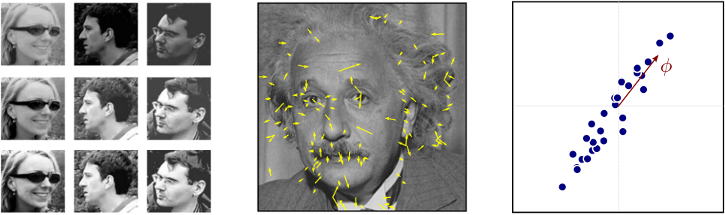
\includegraphics[width=8cm]{figures/intro-collage.png}}
    {\centering Images from \cite{prince12}}
\end{center}

\end{frame}

% -----------------------------------------------------------------------------

\begin{frame}
\frametitle{What Is CV and Why Is It Important?}

Let's hear what Fei-Fei Li has to say

\bigskip
\begin{center}
    \copyrightbox[b]
    {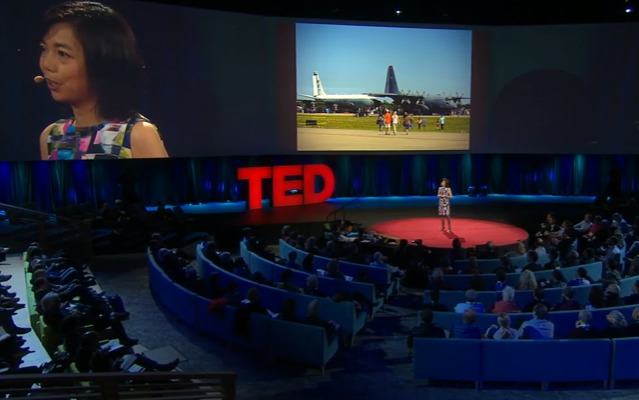
\includegraphics[width=7cm]{figures/feifei-ted.jpg}}
    {\centering Image from \href{https://www.ted.com/talks/fei_fei_li_how_we_re_teaching_computers_to_understand_pictures}{\texttt{ted.com}}}
\end{center}

\end{frame}

% -----------------------------------------------------------------------------

\begin{frame}
\frametitle{What Is CV and Why Is It Important?}

CV is about making computers understand images like humans do\\\medskip
Key to novel autonomous systems (cars, security, data analysis)\\\medskip
Tremendous progress in last decades, but still unsolved

\end{frame}

% -----------------------------------------------------------------------------

\begin{frame}
\frametitle{CV Past, Present, Future}

CV research started around 50 years ago\\\medskip
Let's take a look at a few examples

\end{frame}

% -----------------------------------------------------------------------------

\begin{frame}
\frametitle{CV Past, Present, Future}
\framesubtitle{1963: Pose Estimation}

Edge-based pose estimation of polyhedra \\\medskip % based on relative orientation of edges
Among first CV applications % but not the first as often claimed, see Steve Seitz's slides

\bigskip
\begin{center}
    \copyrightbox[b]
    {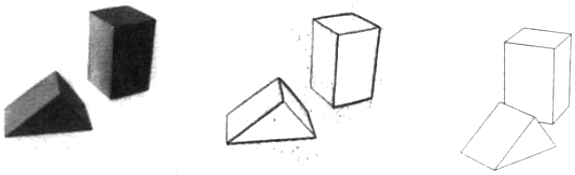
\includegraphics[width=7cm]{figures/blocks-world.png}} % input image, gradient-based edge detection, rendered objects from different viewpoint after recognition
    {\centering Image from \cite{roberts1963}}
\end{center}

\end{frame}

% -----------------------------------------------------------------------------

\begin{frame}
\frametitle{CV Past, Present, Future}
\framesubtitle{1973: Part-Based Object Detection}

Object representation as parts connected by springs\\\medskip % springs illustrate spatial relations
Known as pictorial structures or constellation models % can be solved in polynomial time via DP if the relation graph is a tree / still used today in improved form

\bigskip
\begin{center}
    \copyrightbox[b]
    {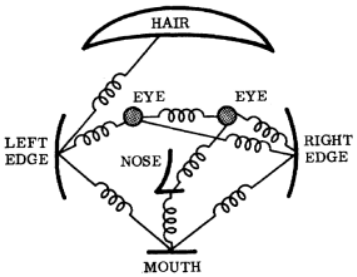
\includegraphics[width=4.5cm]{figures/constellation-model.png}}
    {\centering Image from \cite{fischler1973}}
\end{center}

\end{frame}

% -----------------------------------------------------------------------------

\begin{frame}
\frametitle{CV Past, Present, Future}
\framesubtitle{1989: OCR Using Convolutional Neural Networks}

% good article on DL history: http://www.wired.com/2014/01/geoffrey-hinton-deep-learning

Zip code recognition from images\\\medskip % from US postal service codes, manual preprocessing to obtain one image per digit
Among first applications using convolutional neural networks % but they had been proposed before, see LeCun's paper

\bigskip
\begin{center}
    \copyrightbox[b]
    {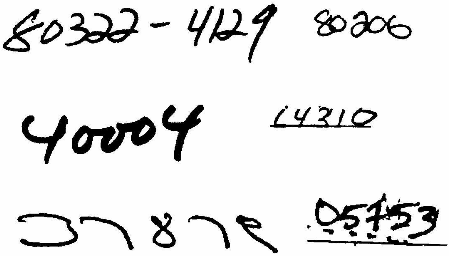
\includegraphics[width=4cm]{figures/zip-numbers.png}}
    {\centering Image from \cite{lecun1989}}
\end{center}

\end{frame}

% -----------------------------------------------------------------------------

\begin{frame}
\frametitle{CV Past, Present, Future}
\framesubtitle{1989: OCR Using Convolutional Neural Networks}

\begin{center}
    \copyrightbox[b]
    {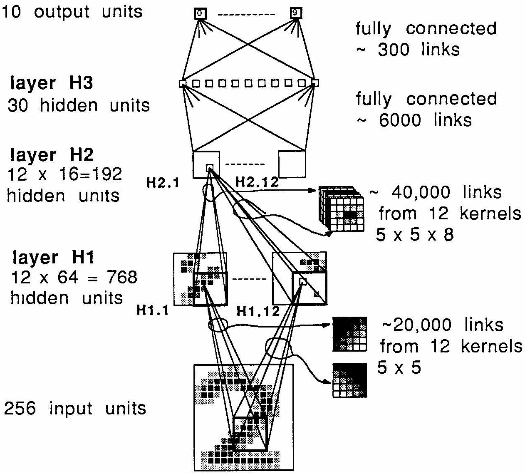
\includegraphics[width=6.5cm]{figures/zip-dnn.png}} % used network architecture. input is 16x16=256, h1 and h2 are convolutional, h3 and output are fully connected. 1256 units, ~65k connections, ~10k params in total
    {\centering Image from \cite{lecun1989}}
\end{center}

\end{frame}

% -----------------------------------------------------------------------------

\begin{frame}
\frametitle{CV Past, Present, Future}
\framesubtitle{1996: Image-Based Modeling}

Generate a 3D model from a set of images\\\medskip
Use this model and input images to render new images\\\medskip
\url{https://www.youtube.com/watch?v=RPhGEiM_6lM} % Facade introduced view-dependent texture mapping (select "best" images for texturing automatically based on similarity of current and image camera view), used for Matrix bullet-time shots according to video description

\bigskip
\begin{center}
    \copyrightbox[b]
    {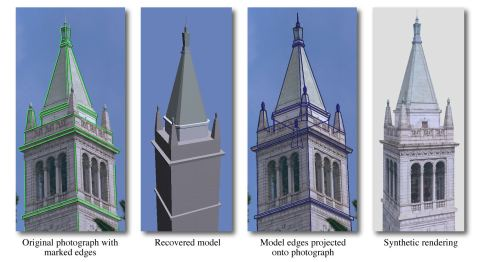
\includegraphics[width=6cm]{figures/facade.jpg}}
    {\centering Images from \cite{debevec1996}}
\end{center}

\end{frame}

% -----------------------------------------------------------------------------

\begin{frame}
\frametitle{CV Past, Present, Future}
\framesubtitle{2001: Real-Time Object Detection}

Fast object detection using Haar features and boosting\\\medskip % feature computation in constant time using integral images
Similar technologies used in smart cameras for auto focus

\bigskip
\begin{center}
    \copyrightbox[b]
    {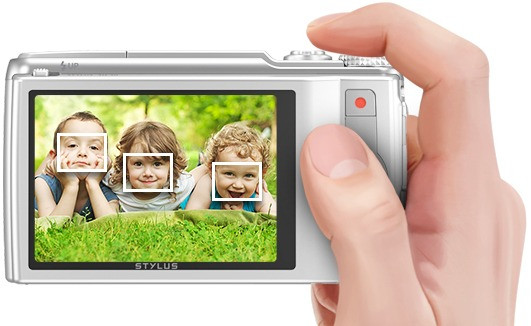
\includegraphics[width=6cm]{figures/camera-faces.jpg}}
    {\centering Image from \url{olympus-europa.com}}
\end{center}

\end{frame}

% -----------------------------------------------------------------------------

\begin{frame}
\frametitle{CV Past, Present, Future}
\framesubtitle{2006: Photo Tourism}

3D reconstruction from photo collections\\\medskip
Structure from Motion (SIFT + bundle adjustment) % these things were developed earlier

\bigskip
\begin{center}
    \copyrightbox[b]
    {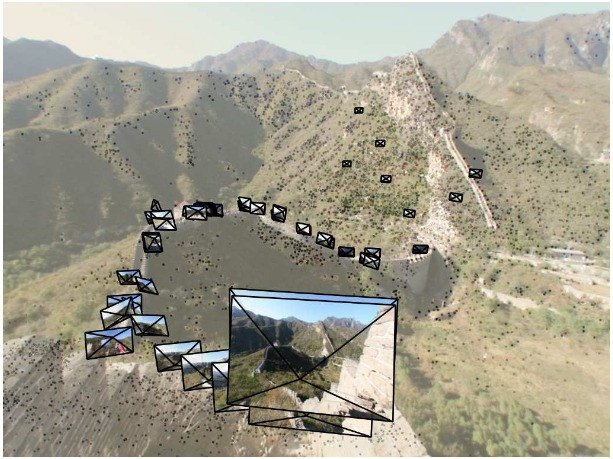
\includegraphics[width=5cm]{figures/photo-tourism.jpg}}
    {\centering Image from \cite{snavely2006}}
\end{center}

\end{frame}

% -----------------------------------------------------------------------------

\begin{frame}
\frametitle{CV Past, Present, Future}
\framesubtitle{2006: Photo Tourism -- Microsoft Photosynth}

\begin{center}
    \copyrightbox[b]
    {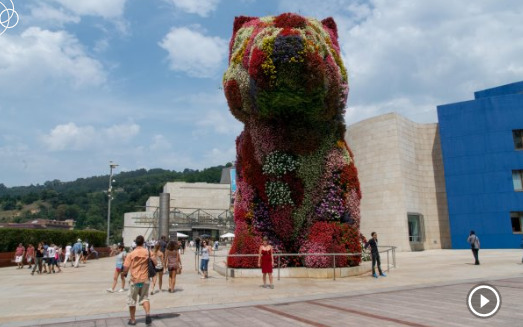
\includegraphics[width=7cm]{figures/photosynth.jpg}}
    {\centering Image from \href{https://photosynth.net/}{\texttt{photosynth.net}}}
\end{center}

\end{frame}

% -----------------------------------------------------------------------------

\begin{frame}
\frametitle{CV Past, Present, Future}
\framesubtitle{2006: Photo Tourism -- Building Rome in a Day}

\begin{center}
    \copyrightbox[b]
    {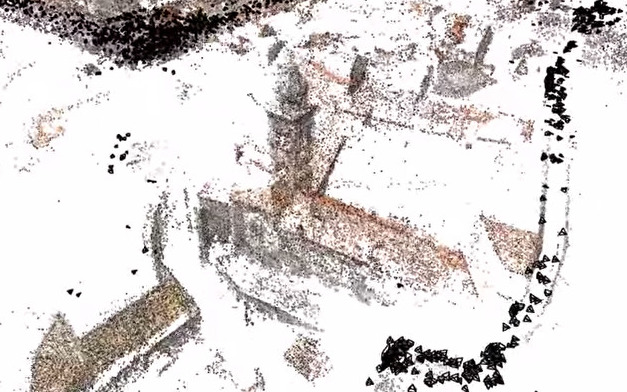
\includegraphics[width=7cm]{figures/dubrovnik.jpg}}
    {\centering Image from \url{https://www.youtube.com/watch?v=sQegEro5Bfo}}
\end{center}

\end{frame}

% -----------------------------------------------------------------------------

\begin{frame}
\frametitle{CV Past, Present, Future}
\framesubtitle{2011: Kinect}

Depth estimation via active stereo\\\medskip
Real-time pose estimation of multiple players

\bigskip
\begin{center}
    \copyrightbox[b]
    {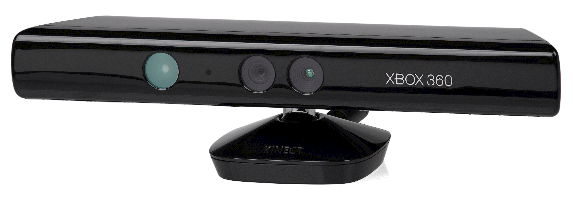
\includegraphics[width=5cm]{figures/kinect.png}}
    {\centering Image from \url{wikipedia.org}}
    \qquad
    \copyrightbox[b]
    {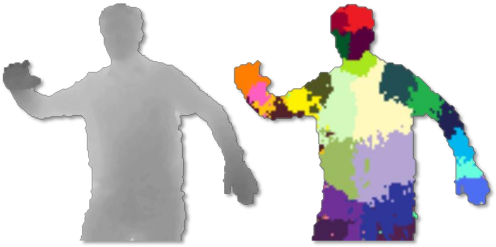
\includegraphics[width=4cm]{figures/kinect-pose.png}}
    {\centering Image from \cite{shotton2011}}
\end{center}

\end{frame}

% -----------------------------------------------------------------------------

\begin{frame}
\frametitle{CV Past, Present, Future}
\framesubtitle{2012: Deep Learning and Big Data}

Deep Learning on huge datasets for object recognition

\bigskip
\begin{center}
    \copyrightbox[b]
    {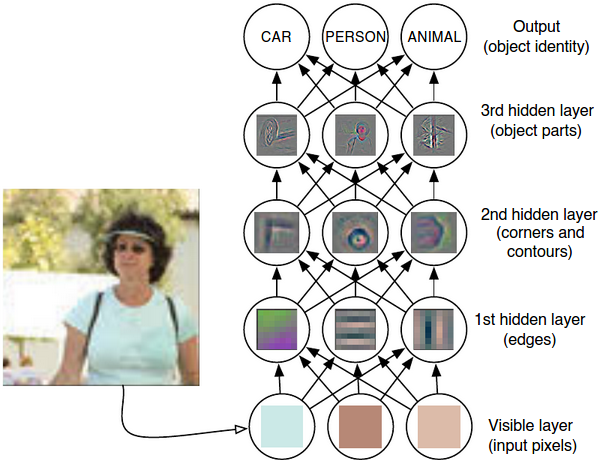
\includegraphics[width=6cm]{figures/dl-layer-example}}
    {\centering Image from \cite{bengio2015}}
\end{center}

\end{frame}

% -----------------------------------------------------------------------------

\begin{frame}
\frametitle{CV Past, Present, Future}
\framesubtitle{2012: Deep Learning and Big Data -- Clarifai}

% continue Fei-Fei Li's talk

\bigskip
\begin{center}
    \copyrightbox[b]
    {
\includegraphics[width=7cm]{figures/clarifai.jpg}}
    {\centering Image from \href{http://www.clarifai.com}{\texttt{clarifai.com}}}
\end{center}

\end{frame}

% -----------------------------------------------------------------------------

\begin{frame}
\frametitle{CV Past, Present, Future}
\framesubtitle{2012: Deep Learning and Big Data}

% continue Fei-Fei Li's talk

\bigskip
\begin{center}
    \copyrightbox[b]
    {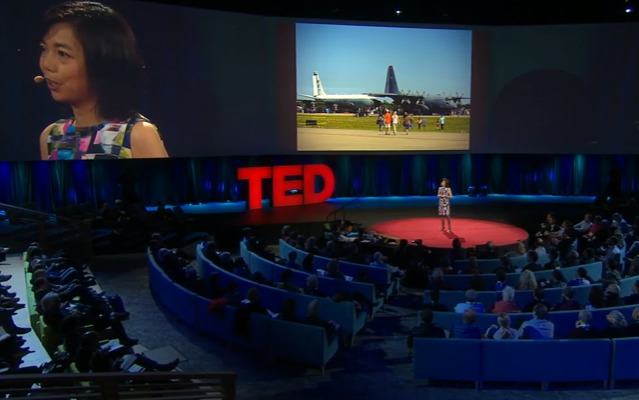
\includegraphics[width=7cm]{figures/feifei-ted.jpg}}
    {\centering Image from \href{https://www.ted.com/talks/fei_fei_li_how_we_re_teaching_computers_to_understand_pictures}{\texttt{ted.com}}}
\end{center}

\end{frame}

% -----------------------------------------------------------------------------

\begin{frame}
\frametitle{CV Past, Present, Future}
\framesubtitle{20xx: Human-Level Object Recognition}

Object recognition without constraints % like occlusions, perspective, background

\bigskip
\begin{center}
    \copyrightbox[b]
    {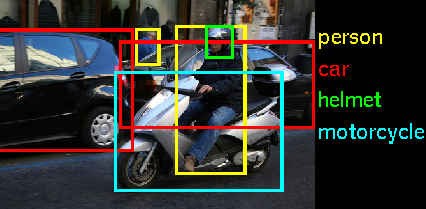
\includegraphics[width=6cm]{figures/object-detection.png}}
    {\centering Image from \url{image-net.org}}
\end{center}

\end{frame}

% -----------------------------------------------------------------------------

\begin{frame}
\frametitle{CV Past, Present, Future}
\framesubtitle{20xx: Autonomous Cars}

Cars that drive autonomously\\\medskip
\url{https://www.youtube.com/watch?v=bDOnn0-4Nq8}

\bigskip
\begin{center}
    \copyrightbox[b]
    {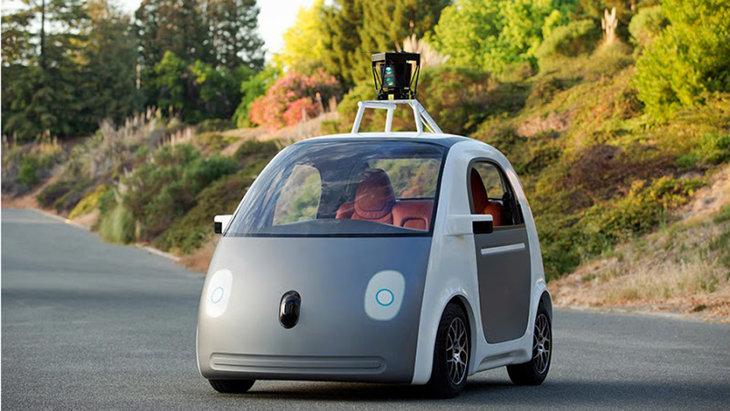
\includegraphics[width=6cm]{figures/google-car.jpg}}
    {\centering Image by Google}
\end{center}

\end{frame}

% -----------------------------------------------------------------------------

\begin{frame}
\frametitle{CV Past, Present, Future}
\framesubtitle{20xx: Human-Level Vision}

Segmentation, context, motion, emotions

\bigskip
\begin{center}
    \copyrightbox[b]
    {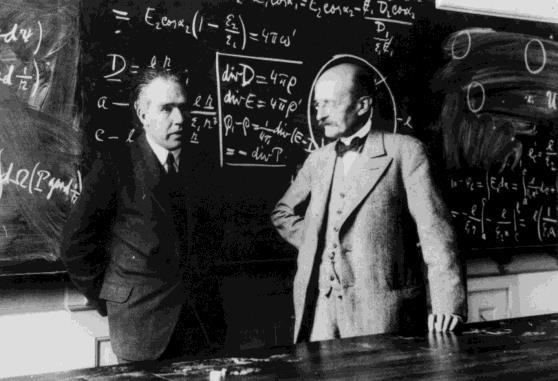
\includegraphics[width=6cm]{figures/planck-bohr.png}}
    {\centering Image from Larry Zitnick's slides}
\end{center}

\end{frame}

% -----------------------------------------------------------------------------

\begin{frame}
\frametitle{CV Past, Present, Future}
\framesubtitle{20xx: Human-Level Vision}

% continue Fei-Fei Li's talk

\bigskip
\begin{center}
    \copyrightbox[b]
    {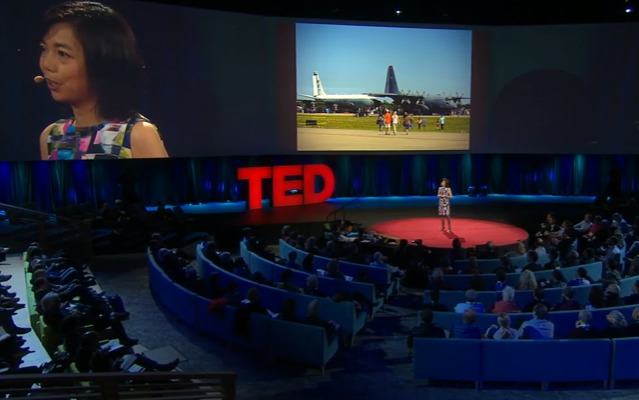
\includegraphics[width=7cm]{figures/feifei-ted.jpg}}
    {\centering Image from \href{https://www.ted.com/talks/fei_fei_li_how_we_re_teaching_computers_to_understand_pictures}{\texttt{ted.com}}}
\end{center}

\end{frame}

% -----------------------------------------------------------------------------

{
\setbeamertemplate{footline}{}
\begin{frame}

% show one of my photos as a filler just to break up the presentation to indicate a new chapter

\begin{tikzpicture}[remember picture,overlay]
    \node[at=(current page.center)] {
        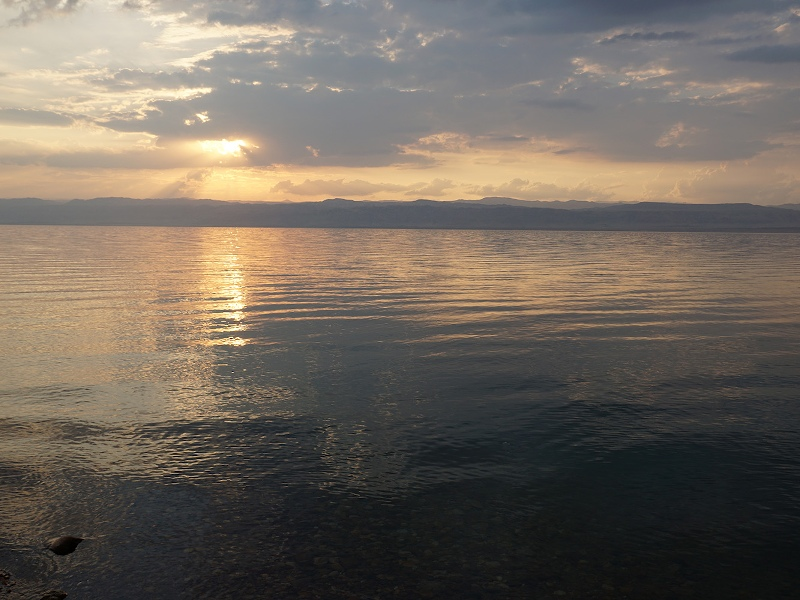
\includegraphics[width=\paperwidth]{figures/dead-sea.jpg}
    };
    \node[at=(current page.center),align=center,yshift=-4cm,gray] {\footnotesize Dead Sea, Jordan, 2014};
\end{tikzpicture}

\end{frame}
}

% -----------------------------------------------------------------------------

\begin{frame}
\frametitle{CV and Related Fields}

In other lectures you probably heard about
\begin{itemize}
    \item Mathematics and statistics
    \item Image processing (e.g.\ linear filtering, SIFT)
    \item Machine learning (e.g.\ SVM)
\end{itemize}

\bigskip
Let's see how CV and these fields are related

\end{frame}

% -----------------------------------------------------------------------------

\begin{frame}
\frametitle{CV and Related Fields}
\framesubtitle{Formal Definition of CV}

CV is about making computers understand images like humans do

\bigskip
So in mathematical terms CV is about
\begin{itemize}
    \item Inferring some world state (a scalar $w$ or vector $\vw$)
    \item From measurements $\vx$ (a \emph{feature vector})
\end{itemize}

\end{frame}

% -----------------------------------------------------------------------------

\begin{frame}
\frametitle{CV and Related Fields}
\framesubtitle{Image Processing}

We use \emph{image processing} to extract $\vx$ from images
\begin{itemize}
    \item Preprocessing step for CV
    \item Different problems favor different $\vx$
\end{itemize}

\end{frame}

% -----------------------------------------------------------------------------

\begin{frame}
\frametitle{CV and Related Fields}
\framesubtitle{Image Processing}

Example: scene category classification
\begin{itemize}
    \item $\vx$ : histogram of SIFT visual words
    \item $w$ : scene class label (e.g.\ desert, jungle)
\end{itemize}

\begin{center}
    \copyrightbox[b]
    {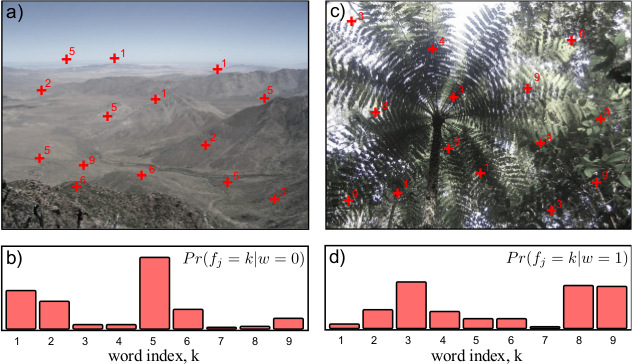
\includegraphics[width=6cm]{figures/visual-words.jpg}}
    {\centering Image from \cite{prince12}}
\end{center}

\end{frame}

% -----------------------------------------------------------------------------

\begin{frame}
\frametitle{CV and Related Fields}
\framesubtitle{Statistics}

CV is about inferring some world state $\vw$ from measurements $\vx$

\bigskip
And thus about describing the relationship between $\vx$ and $\vw$
\begin{itemize}
    \item This relationship is called \emph{model}
\end{itemize}

\bigskip
Models are ideally statistical (probabilistic)
\begin{itemize}
    \item Allow us to reason about uncertainty
\end{itemize}

\end{frame}

% -----------------------------------------------------------------------------

\begin{frame}
\frametitle{CV and Related Fields}
\framesubtitle{Statistics}

Statistical analysis can help select a suitable model % especially for low feature dimensionalities

\bigskip
\begin{center}
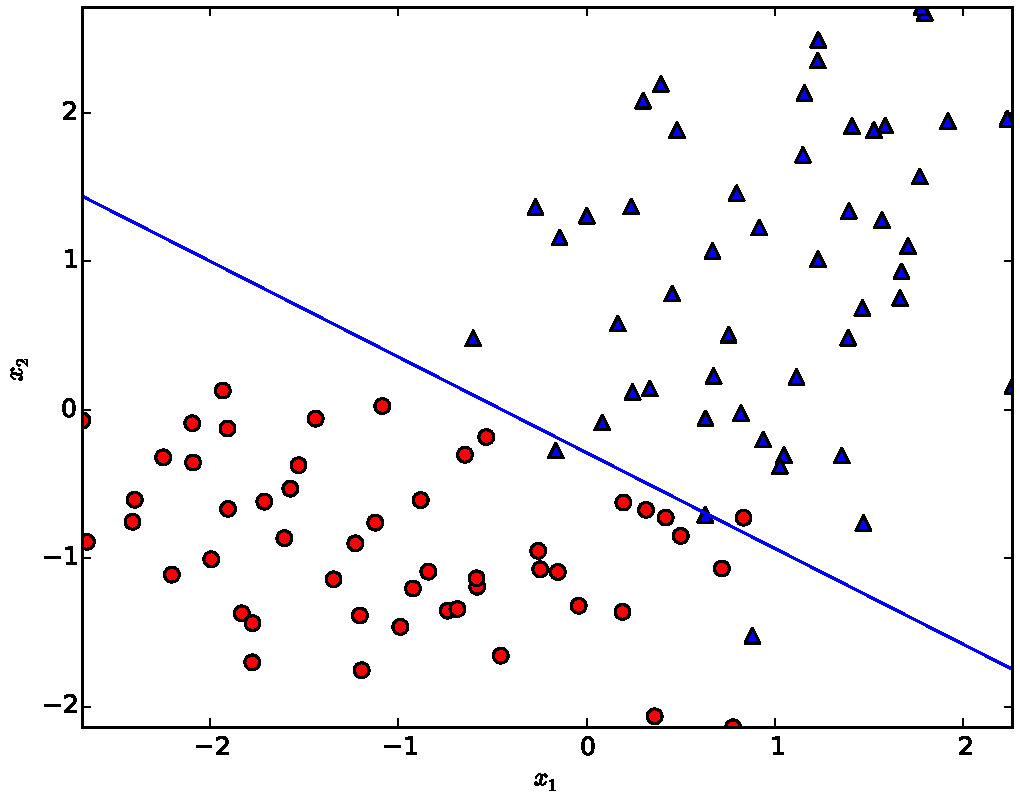
\includegraphics[width=6cm]{figures/perceptron-classification.pdf} % in this example a visualization of x and w suggests that the two classes are linearly separated apart from noise and a few outliers, so a linear model would be a good choice
\end{center}

\end{frame}

% -----------------------------------------------------------------------------

\begin{frame}
\frametitle{CV and Related Fields}
\framesubtitle{Mathematics}

\bigskip
A model usually has two kinds of \emph{parameters}
\begin{itemize}
    \item \emph{Hyperparameters} that are set manually
    \item Parameters $\pv$ that are \emph{learned} from data
\end{itemize}

\bigskip
Learning involves finding a $\pv$ that
\begin{itemize}
    \item Minimizes the disagreement (\emph{loss}) between $\dot{\vw}$ and $\vw$ % average loss. this is often not possible because finding the global minimum can be impractical. good local minima often suffice though. the loss function must be defined depending on the task
    \item Given \emph{training samples} $\{(\vx,\dot{\vw})\}$ and predictions $\vw=\Gamma(\vx;\pv)$ % in the supervised case, but let's skip these details for
\end{itemize}

\bigskip
This is a \emph{mathematical optimization} problem

\end{frame}

% -----------------------------------------------------------------------------

\begin{frame}
\frametitle{CV and Related Fields}
\framesubtitle{Machine Learning}

\emph{Machine Learning} (ML) studies techniques for learning from data
\begin{itemize}
    \item Namely algorithms for learning and inference
    \item So any CV model that involves learning is a ML technique
\end{itemize}

\bigskip
CV often makes use of generic ML algorithms (e.g.\ SVM) % unless we know the physical relationship between x and v e.g. structure from motion, tracking with sensor noise

\bigskip
Strictly speaking, models and algorithms are not the same
\begin{itemize}
    \item More on this later
\end{itemize}

\end{frame}

% -----------------------------------------------------------------------------

{
\setbeamertemplate{footline}{}
\begin{frame}

% show one of my photos as a filler just to break up the presentation to indicate a new chapter

\begin{tikzpicture}[remember picture,overlay]
    \node[at=(current page.center)] {
        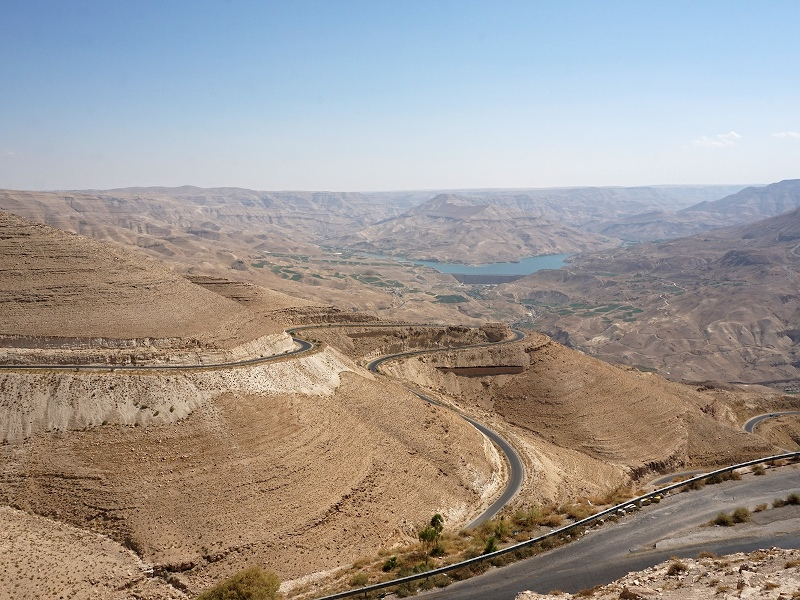
\includegraphics[width=\paperwidth]{figures/wadi-mujib.jpg}
    };
    \node[at=(current page.center),align=center,yshift=-4cm,white] {\footnotesize Wadi Mujib, Jordan, 2014};
\end{tikzpicture}

\end{frame}
}

% -----------------------------------------------------------------------------

\begin{frame}
\frametitle{Image Processing Recap}

We use Image Processing (IP) to extract a suitable $\vx$ from images
\begin{itemize}
    \item IP has great influence on CV performance
\end{itemize}

\bigskip
Suitable means
\begin{itemize}
    \item \emph{Distinctive} features % like the two features in the above graph
    \item That are \emph{invariant} and \emph{robust}
\end{itemize}

\bigskip
Such features vary significantly (only) with $w$
\begin{itemize}
    \item So different problems favor different $\vx$
\end{itemize}

\end{frame}

% -----------------------------------------------------------------------------

\begin{frame}
\frametitle{Image Processing Recap}

More on feature selection later

\bigskip
Let's recap some generic IP methods for
\begin{itemize}
    \item Gaining robustness to noise
    \item Detecting brightness changes
    \item Detecting interest points in images
    \item Describing image patches in an invariant way
\end{itemize}

\end{frame}

% -----------------------------------------------------------------------------

\begin{frame}
\frametitle{Image Processing Recap}
\framesubtitle{Noise Reduction}

Gain robustness to noise via blurring

\bigskip
Often accomplished via \emph{linear filtering}
\begin{itemize}
    \item Pixel values linear combination of neighbor values
    \item Computed via \emph{convolution} (or correlation) with kernel $h$
\end{itemize}

\[
f'(x,y) = \sum_{i,j}f(x-i,y-j)h(i,j) % with convolution the kernel is flipped (x-i,y-j), with correlation this is not the case (x+i,y+j) ... most IP kernels are symmetric so the result is the same
\]

\end{frame}

% -----------------------------------------------------------------------------

\begin{frame}
\frametitle{Image Processing Recap}
\framesubtitle{Noise Reduction}

For blurring use a 2D Gaussian as kernel $h$: % there are of course others as well
\[
h(i,j)=\frac{1}{2\pi\sigma^2}\exp\left(-\frac{i^2+j^2}{2\sigma^2}\right)
\]

\begin{center}
    \copyrightbox[b]
    {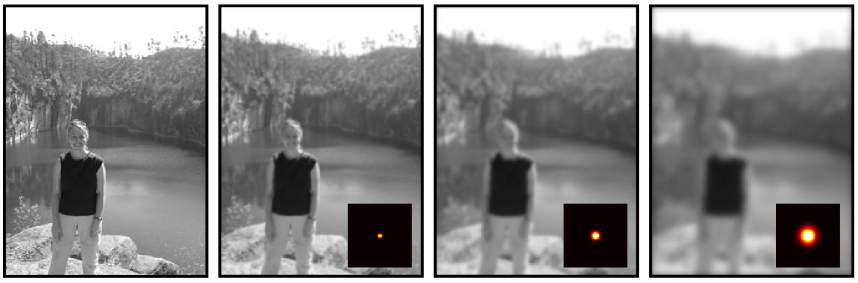
\includegraphics[width=8cm]{figures/linear-blur.png}}
    {\centering Images from \cite{prince12}}
\end{center}

\end{frame}

% -----------------------------------------------------------------------------

\begin{frame}
\frametitle{Image Processing Recap}
\framesubtitle{Detecting Brightness Changes -- LoG Filter}

Brightness changes can be valuable information
\begin{itemize}
    \item Object boundaries, textured regions
\end{itemize}

\bigskip
Use a Laplacian of Gaussian (LoG) filter as kernel $h$ % for 3x3 this is just [0 -1 0 ; -1 4 -1 ; 0 -1 0]
\begin{itemize}
    \item Gaussian for noise reduction
    \item Laplacian approximates $\nabla^2=f_{xx}+f_{yy}$ % sum of second unmixed derivatives of image
\end{itemize}

\bigskip
LoG filters respond to intensity changes % strong response near corners, zero crossing on corners
\begin{itemize}
    \item Regardless of direction
    \item At a frequency defined by $\sigma$ of Gaussian
\end{itemize}

\end{frame}

% -----------------------------------------------------------------------------

\begin{frame}
\frametitle{Image Processing Recap}
\framesubtitle{Detecting Brightness Changes -- LoG Filter}

\begin{center}
    \copyrightbox[b]
    {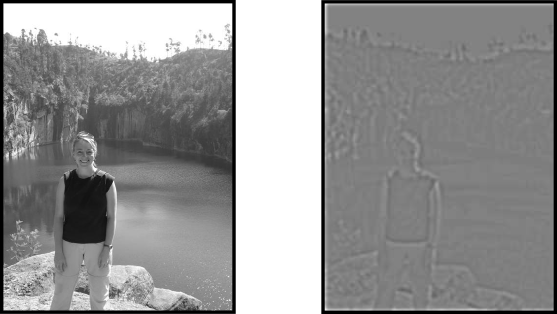
\includegraphics[width=7cm]{figures/linear-log.png}}
    {\centering Images from \cite{prince12}}
\end{center}

\end{frame}

% -----------------------------------------------------------------------------

\begin{frame}
\frametitle{Image Processing Recap}
\framesubtitle{Detecting Brightness Changes -- Gabor Filter}

Direction of brightness changes can be valuable information
\begin{itemize}
    \item Texture information
\end{itemize}

\bigskip
Use a Gabor filter as kernel $h$, which consists of
\begin{itemize}
    \item A Gaussian for noise reduction
    \item A Sinusoid for change detection 
\end{itemize}

\bigskip
Gabor filters respond to intensity changes at a
\begin{itemize}
    \item Phase and orientation defined by the Sinusoid % phase, orientation, wavelength, but can be made independent of phase by summing squared responses of two filters with pi/2 phase shift
    \item Frequency defined by the Gaussian and Sinusoid
\end{itemize}

\end{frame}

% -----------------------------------------------------------------------------

\begin{frame}
\frametitle{Image Processing Recap}
\framesubtitle{Detecting Brightness Changes -- Gabor Filter}

\begin{center}
    \copyrightbox[b]
    {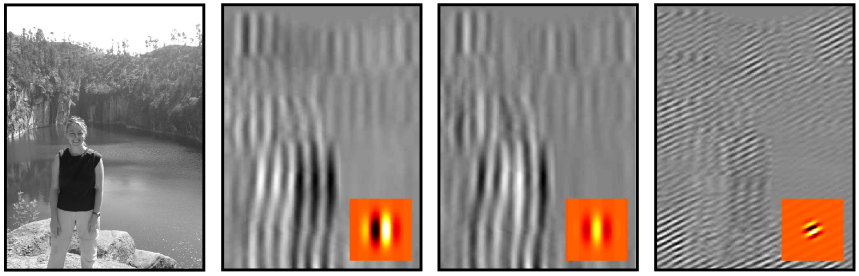
\includegraphics[width=10cm]{figures/linear-gabor.png}}
    {\centering Images from \cite{prince12}}
\end{center}

\end{frame}

% -----------------------------------------------------------------------------

\begin{frame}
\frametitle{Image Processing Recap}
\framesubtitle{Interest Point Detection}

\emph{Interest points} (keypoints) are
\begin{itemize}
    \item Distinctive locations in images
    \item Invariant and robust to image transformations % depending on the type of keypoint
\end{itemize}

\bigskip
Can be detected reliably in multiple images of same object
\begin{itemize}
    \item Used for object detection, structure from motion
\end{itemize}

\end{frame}

% -----------------------------------------------------------------------------

\begin{frame}
\frametitle{Image Processing Recap}
\framesubtitle{Interest Point Detection -- Harris}

Corners characterized by intensity change in multiple directions

\bigskip
Harris corner detector exploits this by
\begin{itemize}
    \item Checking gradient distribution in local neighborhood
    \item Corner: gradient distribution has two large eigenvalues
\end{itemize}

\begin{center}
    \copyrightbox[b]
    {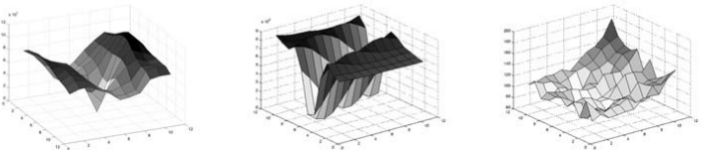
\includegraphics[width=10cm]{figures/cornerness.png}}
    {\centering Images from \cite{szeliski2010}}
\end{center}

\end{frame}

% -----------------------------------------------------------------------------

\begin{frame}
\frametitle{Image Processing Recap}
\framesubtitle{Interest Point Detection -- Harris}

Harris interest points
\begin{itemize}
    \item Are invariant to translation and rotation
    \item Stable under varying lighting conditions % because they are based on derivatives
\end{itemize} % they are also among the most repeatable and most informative, see Tuytelaars08

\medskip
\begin{center}
    \copyrightbox[b]
    {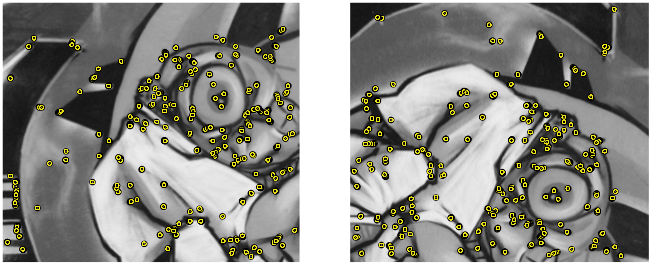
\includegraphics[width=8cm]{figures/ip-harris.png}}
    {\centering Images from \cite{tuytelaars2008}}
\end{center}

\end{frame}

% -----------------------------------------------------------------------------

\begin{frame}
\frametitle{Image Processing Recap}
\framesubtitle{Interest Point Detection -- SIFT}

Scale invariant blob detector
\begin{itemize}
    \item A blob is an image region with similar intensity % surrounded by regions with different intensity, again see Tuytelaars08 for more information
\end{itemize}

\bigskip
Blob detection accomplished via LoG filtering
\begin{itemize}
    \item LoG filter responds to blobs of size that depends on $\sigma$
\end{itemize}

\bigskip
Scale invariance is achieved by
\begin{itemize}
    \item Applying LoG filter with multiple $\sigma$
    \item Finding local maxima in resulting scale-space
\end{itemize}

\bigskip
Repeated LoG approximated by Differences of Gaussians (DoGs)

\end{frame}

% -----------------------------------------------------------------------------

\begin{frame}
\frametitle{Image Processing Recap}
\framesubtitle{Interest Point Detection -- SIFT Scale Space}

\begin{center}
    \copyrightbox[b]
    {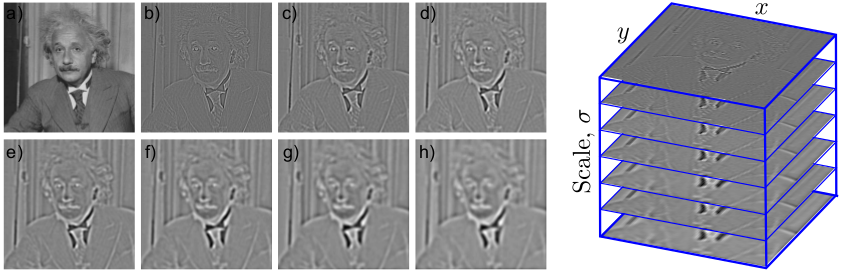
\includegraphics[width=10cm]{figures/sift-scale-space.png}}
    {\centering Images from \cite{prince12}}
\end{center}

\end{frame}

% -----------------------------------------------------------------------------

\begin{frame}
\frametitle{Image Processing Recap}
\framesubtitle{Interest Point Detection -- SIFT}

Local maxima are
\begin{itemize}
    \item Localized to sub-voxel accuracy % via Taylor expansion, which leads to a more accurate position and scale estimation, see Prince's book
    \item Discarded unless on corners % corners in the above sense, not necessarily actual corners
    \item Assigned an orientation via gradient histograms % multiple keypoints are generated if there are more several dominant orientations
\end{itemize}

\begin{center}
    \copyrightbox[b]
    {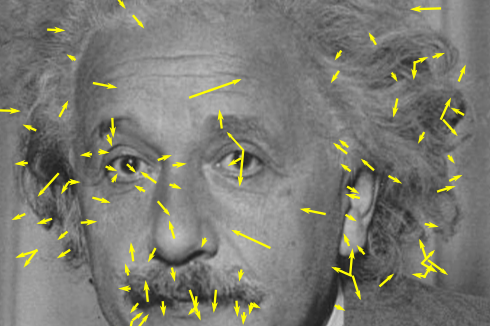
\includegraphics[width=4cm]{figures/ip-sift.png}}
    {\centering Image from \cite{prince12}}
\end{center}

\end{frame}

% -----------------------------------------------------------------------------

\begin{frame}
\frametitle{Image Processing Recap}
\framesubtitle{Local Descriptors}

Compact representations of contents of an image region\\\medskip
Usually computed at interest point locations\\\medskip % but dense representations have uses as well
Invariant in conjunction with suitable interest points\\\medskip % see next slide
Pool information locally to achieve robustness % wrt. small spatial transformations / tradeoff between preserving spatial information and robustness

\end{frame}

% -----------------------------------------------------------------------------

\begin{frame}
\frametitle{Image Processing Recap}
\framesubtitle{Local Descriptors -- SIFT}

Computed from gradient histograms\\\medskip
Usually used together with SIFT interest points
\begin{itemize}
    \item Compensate for scale, rotation % by transforming image patch by interest point properties before computing descriptors
\end{itemize}

\begin{center}
    \copyrightbox[b]
    {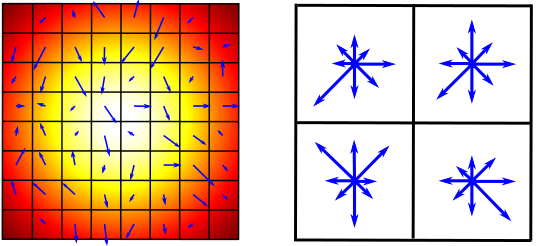
\includegraphics[width=6cm]{figures/sift-descriptor.png}} % divide 8x8 pixel grid into 2x2 cells, pool directions in each cell using a histogram with 8 bins (sift uses 16x16 patches and 4x4 cells, so we have 4x4x8=128 values per descriptor, which is then normalized)
    {\centering Images from \cite{prince12}}
\end{center}

\end{frame}

% -----------------------------------------------------------------------------

\begin{frame}
\frametitle{Image Processing Recap}
\framesubtitle{Local Descriptors -- SIFT}

SIFT descriptors are
\begin{itemize}
    \item Invariant to scale and rotation (interest points)
    \item Invariant to global intensity changes (gradients)
    \item Robust to small affine transformations (pooling)
\end{itemize}

\end{frame}

% -----------------------------------------------------------------------------

\begin{frame}[allowframebreaks=0.9]
\frametitle{Bibliography}

\printbibliography

\end{frame}

\end{document}
